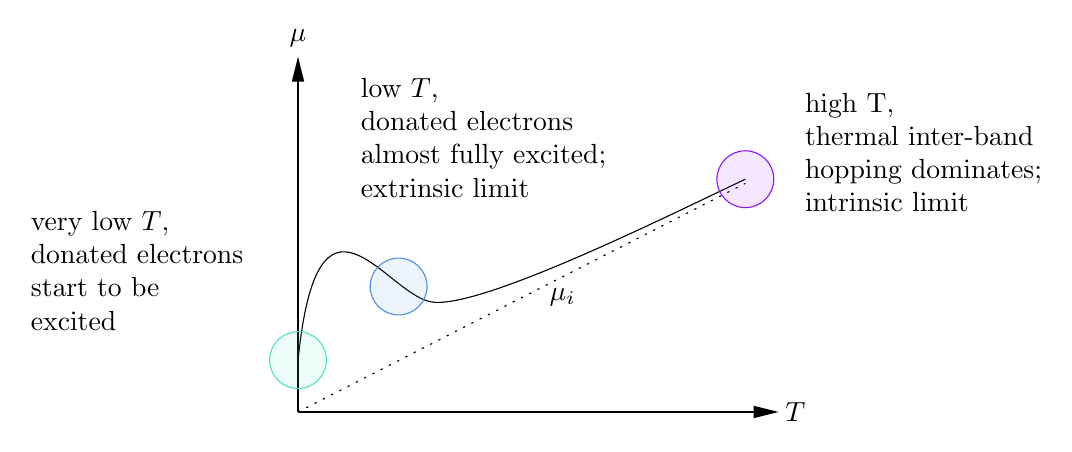
\begin{tikzpicture}[x=0.75pt,y=0.75pt,yscale=-1,xscale=1]
    %uncomment if require: \path (0,355); %set diagram left start at 0, and has height of 355
    
    %Straight Lines [id:da12533057960173433] 
    \draw    (150,224) -- (379.5,224) ;
    \draw [shift={(381.5,224)}, rotate = 180] [fill={rgb, 255:red, 0; green, 0; blue, 0 }  ][line width=0.08]  [draw opacity=0] (12,-3) -- (0,0) -- (12,3) -- cycle    ;
    %Straight Lines [id:da46025762315895236] 
    \draw    (150,224) -- (150,54.85) ;
    \draw [shift={(150,52.85)}, rotate = 90] [fill={rgb, 255:red, 0; green, 0; blue, 0 }  ][line width=0.08]  [draw opacity=0] (12,-3) -- (0,0) -- (12,3) -- cycle    ;
    %Straight Lines [id:da9241041282655598] 
    \draw  [dash pattern={on 0.84pt off 2.51pt}]  (150,224) -- (365.5,113.85) ;
    %Curve Lines [id:da902430446942259] 
    \draw    (150,199) .. controls (159.5,104.85) and (191.5,165.85) .. (213.5,170.85) .. controls (235.5,175.85) and (329.5,128.85) .. (365.5,111.85) ;
    %Shape: Circle [id:dp16809872568107043] 
    \draw  [color={rgb, 255:red, 80; green, 227; blue, 194 }  ,draw opacity=1 ][fill={rgb, 255:red, 80; green, 227; blue, 194 }  ,fill opacity=0.1 ] (136.3,199) .. controls (136.3,191.43) and (142.43,185.3) .. (150,185.3) .. controls (157.57,185.3) and (163.7,191.43) .. (163.7,199) .. controls (163.7,206.57) and (157.57,212.7) .. (150,212.7) .. controls (142.43,212.7) and (136.3,206.57) .. (136.3,199) -- cycle ;
    %Shape: Circle [id:dp2672422180325582] 
    \draw  [color={rgb, 255:red, 74; green, 144; blue, 226 }  ,draw opacity=1 ][fill={rgb, 255:red, 74; green, 144; blue, 226 }  ,fill opacity=0.1 ] (184.75,163.55) .. controls (184.75,155.99) and (190.88,149.85) .. (198.45,149.85) .. controls (206.01,149.85) and (212.15,155.99) .. (212.15,163.55) .. controls (212.15,171.12) and (206.01,177.25) .. (198.45,177.25) .. controls (190.88,177.25) and (184.75,171.12) .. (184.75,163.55) -- cycle ;
    %Shape: Circle [id:dp6203728259149861] 
    \draw  [color={rgb, 255:red, 144; green, 19; blue, 254 }  ,draw opacity=1 ][fill={rgb, 255:red, 144; green, 19; blue, 254 }  ,fill opacity=0.1 ] (351.8,111.85) .. controls (351.8,104.29) and (357.93,98.16) .. (365.5,98.16) .. controls (373.07,98.16) and (379.2,104.29) .. (379.2,111.85) .. controls (379.2,119.42) and (373.07,125.55) .. (365.5,125.55) .. controls (357.93,125.55) and (351.8,119.42) .. (351.8,111.85) -- cycle ;
    
    % Text Node
    \draw (270,163.4) node [anchor=north west][inner sep=0.75pt]    {$\mu _{\text{i}}$};
    % Text Node
    \draw (383.5,224) node [anchor=west] [inner sep=0.75pt]    {$T$};
    % Text Node
    \draw (150,49.45) node [anchor=south] [inner sep=0.75pt]    {$\mu $};
    % Text Node
    \draw (20,126) node [anchor=north west][inner sep=0.75pt]   [align=left] {very low $\displaystyle T$,\\donated electrons\\start to be \\excited};
    % Text Node
    \draw (179,62) node [anchor=north west][inner sep=0.75pt]   [align=left] {low $\displaystyle T$,\\donated electrons\\almost fully excited;\\extrinsic limit};
    % Text Node
    \draw (393,69) node [anchor=north west][inner sep=0.75pt]   [align=left] {high T,\\thermal inter-band\\hopping dominates;\\intrinsic limit};
    
    
    \end{tikzpicture}
    